\chapter{Modulares Eingabesystem}
\section{Projektbeschreibung}\label{sec:vision}
Das Eingabesystem verfolgt die Vision eines flexiblen und erweiterbaren Systems, das sich an die individuellen Bedürfnisse der Benutzer anpasst. Im Zentrum steht ein Hauptmodul, das als Mikrocontroller-Einheit dient und über eine USB-Schnittstelle mit einem Computer verbunden wird. Dieses Hauptmodul koordiniert die Kommunikation und Funktionalität der verbundenen Module.
\\
\\
Die Module, wie ein Tastatur-Modul mit einer 4x4-Tastenmatrix oder ein Audio-Modul mit Potentiometern und Fadern, sind frei kombinierbar und können je nach Anwendungsfall hinzugefügt oder entfernt werden. Dies ermöglicht eine Konfiguration für unterschiedliche Aufgaben wie Textverarbeitung, Bildbearbeitung, Audiobearbeitung oder Gaming.
\\
\\
In Abbildung xxx ist ein Überblick des Eingabesystems zu sehen:
\begin{figure}[H]
    \centering    
    \fbox{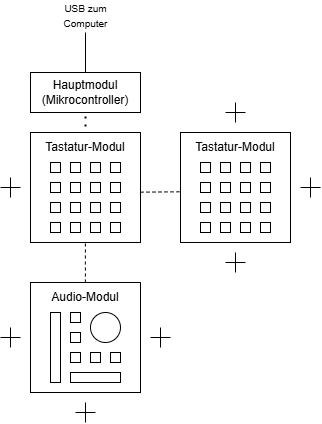
\includegraphics[width=.75\textwidth]{Bilder/bu_vision.png}}
    \caption{Vereinfachte Darstellung des Eingabesystems}
    \label{vision}
\end{figure}
\noindent Die gestrichelten Linien stellen eine bereits hergestellte Verbindung zwischen den Modulen dar, wobei die \glqq Plus\grqq{} Symbole einen weiteren möglichen Modulanschluss darstellen. Die Module sollen fest aneinander sitzen.

\subsection{Verbindung}
Zwischen den Modulen werden Daten und Spannungsversorgung über eine 4 Pin-Verbindung realisiert. Diese sind VCC (Spannungsversorgung), Data + (Datenbus), Data - (invertierter Datenbus) und GND (Masse). Da der Benutzer die Möglichkeit haben soll, jedes Modul an jede Seite eines anderen anstecken zu können, werden pro Seite zwei 2-Pin Pogo Stecker verwendet, ein 2-Pin Male und ein 2-Pin Female Stecker. Dadurch ist das System in jede Richtung erweiterbar. Um eine feste Verbindung zu gewährleisten,  werden Neodym-Magnete ins Gehäuse verbaut. Dies stellt sicher, dass die Pins sicher miteinander verbunden sind und Kontakt haben. 
\begin{figure}[H]
    \centering    
    \fbox{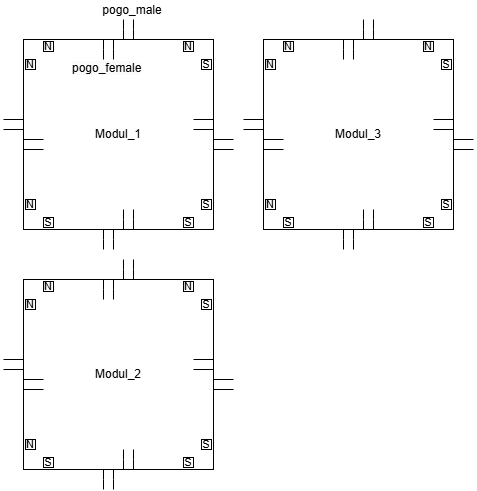
\includegraphics[width=.85\textwidth]{Bilder/bu_pogoverbindung.png}}
    \caption{Verbindung der Module durch Pogo-Stecker und Magnete}
    \label{pogo_verbindung}
\end{figure}
 \noindent Abbildung \ref{pogo_verbindung} zeigt, dass die Steckverbindungen eine nahezu beliebige Anordnung der Module zulassen. Durch die Anordnung der Magneten lassen sich nicht alle Module in jeder Beliebigen Anordnung verbinden wie z.B. Oberseite und Oberseite, die aufgrund der physikalischen Eigenschaften der Magnete nicht verbunden werden können. Die \glqq N\grqq{} und \glqq S\grqq{} Symbole stellen die im Gehäuse verbauten Magneten (Nord- und Südpol) zum Zusammenhalt der Module dar.
 
 
 \subsection{Topologien}
 Der Aufbau des Eingabesystems entspricht einer Vermaschten-Topologie. Das verdeutlicht die Abbildung \ref{vision}, denn mit jedem neuen Modul kann auch eine Verbindung zu einem schon vernetzen Modul entstehen. Die Vorteile dieser Topologie sind:
 -x
 -x
 -x
 
 Der BUS hingegen nutzt die Bus-Topologie, alle Teilnehmer sind über eine Zentrale Bus-Verbindung verbunden. Dies hat Vorteile:
 -x
 -x
 -x
 
 
 
 
"Softwaretechnisch" ist das Konzept nach der Stern-Topologie aufgebaut, denn das Hauptmodul (Mikrocontroller) ist eine zentrale Steuereinheit, an die alle anderen Module angeschlossen sind. Die Tastatur-Module und das Audio-Modul sind jeweils direkt an den Bus angebunden. Die Verbindungen laufen sternförmig von dem Hauptmodul zu den einzelnen Modulen. Die Vorteile einer Stern-Topologie in diesem Projekt sind:
\begin{itemize}
    \item \textbf{Skalierbarkeit:} Weitere Module können einfach an die Zentrale angeschlossen werden.
    \item \textbf{Einfache Fehlersuche:} Da jedes Modul eine direkte Verbindung zur Zentrale hat, ist der Ausfall eines Moduls leichter zu diagnostizieren.
    \item \textbf{Zentrale Kontrolle:} Alle Daten laufen durch das Hauptmodul.
\end{itemize}
Wobei nur ein Nachteil festgestellt werden kann:
\begin{itemize}
    \item \textbf{Abhängigkeit:} Fällt das Hauptmodul aus, funktioniert das gesamte System nicht mehr.
\end{itemize}
